\chapter{弦、引力、紧致化与T对偶}

\lectureoverview{一个点粒子基本上可以在任何光滑几何上一致地运动，但量子弦不能。它无穷多的零点振荡依次探测越来越短的尺度上的靶空间，而当这些振荡被恢复时，有效几何会发生变化。要求这一过程具有不动点便给出\(R_{\mu\nu}=0\)，即真空爱因斯坦方程。随后我们从这一一致性条件转向紧致化。一个圆同时提供Kaluza--Klein动量态与弦缠绕态；交换它们便将半径为\(R\)的圆与半径为\(\alpha'/R\)的圆等同起来。}

\section{作为选择原理的一致性}

有两个问题需要回答。为什么引力会出现在弦理论中，以及为什么弦理论远比点粒子力学更不宽容？它们实际上是同一个问题。一个背景几何只有在一根弦能在其上传播而不保留对我们将弦分辨得多么精细的任意依赖时，才是可接受的。

从对照问题开始：一个被约束在光滑弯曲曲面上的点粒子。经典地，它沿测地线运动，即直线的内禀类比。人们可以用许多短线段来近似这一运动，写出差分方程，然后让线段长度趋于零。结果是一个具有良定义连续极限的常微分方程。

量子力学改变的是对历史的求和，而不是结论。我们不再选取一条经典路径，而是在曲面上的路径上对振幅求和。时间可以再次被分成小步，而该极限等价地由弯曲位形空间上的一个Schr\"odinger方程描述。对于光滑曲面，该极限稳定为一个确定的传播子和谱。

\begin{figure}[H]
  \centering
  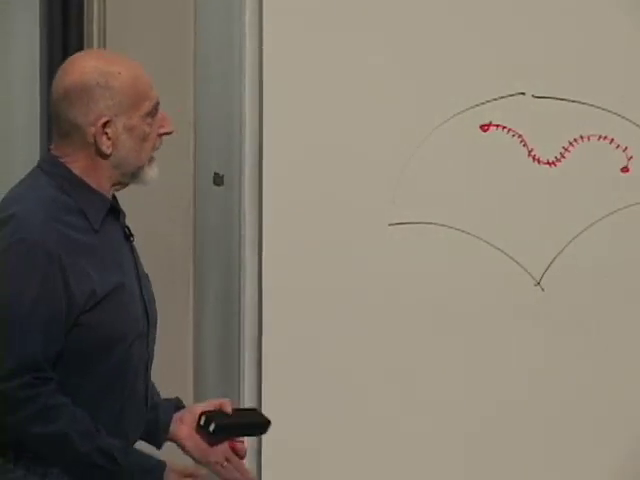
\includegraphics[width=0.72\textwidth]{lecture_09_figure_01.png}
  \caption{曲面上的光滑路径与来自时间切片量子求和的锯齿状路径。二者都保持为靶曲面的内禀对象。}
  \lectureframe{00:05:10}
  \label{fig:l09-particle-paths}
\end{figure}

\begin{classroomqa}
\audiencequestion{在路径积分中，是否要求所有路径都保持在曲面内部？\lecturetimestamp{00:05:39}}
\lecturerresponse{是的。曲面是粒子的位形空间，而不是嵌入在一个更大房间中的一张薄片，粒子不能穿过它走捷径。每一个中间点都属于该曲面，所有长度和作用量都用其内禀度规计算。}
\end{classroomqa}

对于弦，相应的问题更难。一根弦并不仅仅由质心位置来指定。它携带无穷多的振子塔，因此提高分辨率意味着允许更多的动力学自由度。只有当该塔被恢复时观测量趋于一个极限，理论才是一致的。

\section{球面上的点粒子}

球面是最简单的弯曲测试几何。设其半径为\(R\)，并首先将一个质量为\(m\)的粒子置于其上。对于沿大圆的运动，
\begin{equation}
  E=\frac{1}{2}mv^2=\frac{p^2}{2m},
  \qquad
  L=pR.
  \label{eq:l09-particle-energy}
\end{equation}
因此，
\begin{equation}
  E=\frac{L^2}{2mR^2}
   =\frac{L^2}{2I},
  \qquad
  I=mR^2.
  \label{eq:l09-rotor-energy}
\end{equation}
半径通过转动惯量进入。对角动量进行量子化便产生熟悉的刚性转子谱，而没有任何东西依赖于紫外截断。

\begin{figure}[H]
  \centering
  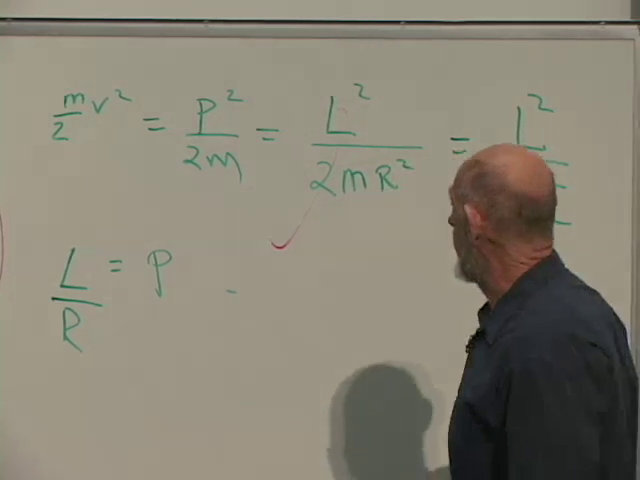
\includegraphics[width=0.74\textwidth]{lecture_09_figure_02.png}
  \caption{点粒子对照计算：
  \(p^2/(2m)=L^2/(2mR^2)=L^2/(2I)\)。}
  \lectureframe{00:11:25}
  \label{fig:l09-sphere-rotor}
\end{figure}

这个毫无困难的例子很重要。曲率本身并不是问题。当曲率与弦的内部量子延展耦合时，问题才出现。

\section{真空弦并非点状}

考虑开弦的一个横向坐标并减去其质心。这里所用的振子展开是示意性的：
\begin{equation}
  X(\sigma)-X_{\mathrm{cm}}
  \sim
  \sum_{n=1}^{\infty}
  \frac{a_n+a_n^\dagger}{\sqrt n}\cos(n\sigma).
  \label{eq:l09-mode-expansion}
\end{equation}
关键要素是余弦模、振子算符以及因子\(1/\sqrt n\)。精确归一化在尺寸论证中不起作用。
\editorialnote{精确展开包含依赖于约定的\(\alpha'\)因子、数值常数以及振子记号的选择。方程\eqref{eq:l09-mode-expansion}只保留了紫外估计所需的依赖关系，正如黑板推导中那样。}

\begin{figure}[H]
  \centering
  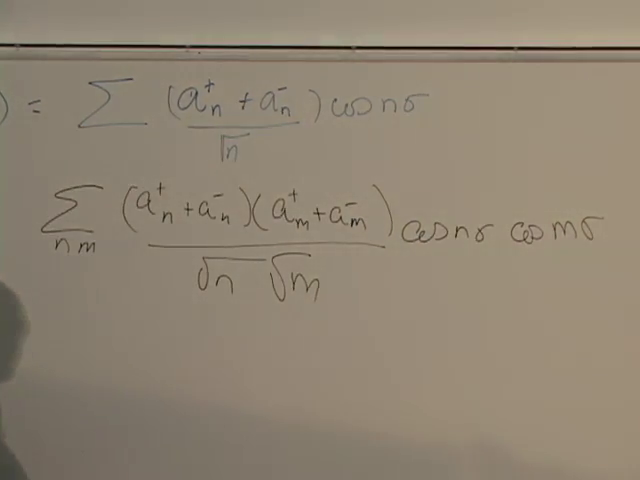
\includegraphics[width=0.78\textwidth]{lecture_09_figure_03.png}
  \caption{结构性的振子展开以及将其平方后得到的双重求和。}
  \lectureframe{00:15:20}
  \label{fig:l09-string-modes}
\end{figure}

在振子真空中，到质心的距离平方为
\begin{align}
  \expect{\bigl(X(\sigma)-X_{\mathrm{cm}}\bigr)^2}_0
  &\sim
  \sum_{n,m\geq1}
  \frac{\cos(n\sigma)\cos(m\sigma)}{\sqrt{nm}}\notag\\
  &\qquad\times
  \bra{0}(a_n+a_n^\dagger)\notag\\
  &\hspace{6em}\times(a_m+a_m^\dagger)\ket{0}.
  \label{eq:l09-size-double-sum}
\end{align}
大多数项都消失。两个湮灭算符将右矢消灭；两个产生算符留下一个与左矢正交的态；而一个产生算符后接一个湮灭算符在这种排序下也有零真空期望值。幸存的收缩为
\begin{equation}
  \bra{0}a_n a_m^\dagger\ket{0}=\delta_{nm}.
  \label{eq:l09-vacuum-contraction}
\end{equation}

\begin{figure}[H]
  \centering
  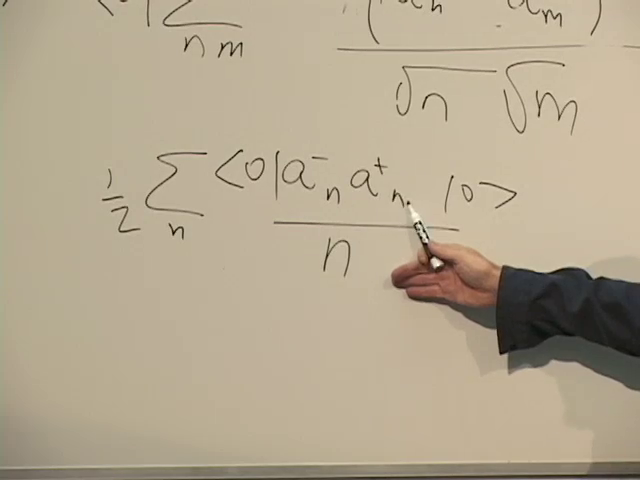
\includegraphics[width=0.74\textwidth]{lecture_09_figure_04.png}
  \caption{存活下来的真空收缩把双振子求和坍缩为单个求和。}
  \lectureframe{00:20:10}
  \label{fig:l09-vacuum-contraction}
\end{figure}

因此
\begin{equation}
  \expect{\bigl(X(\sigma)-X_{\mathrm{cm}}\bigr)^2}_0
  \sim
  \sum_{n=1}^{\infty}\frac{\cos^2(n\sigma)}{n}.
  \label{eq:l09-size-single-sum}
\end{equation}
在弦上的一个一般点处，或在对\(\sigma\)取平均之后，
\(\cos^2(n\sigma)\)大致贡献\(1/2\)。取模式截断
\(N\)，
\begin{equation}
  \expect{\bigl(X-X_{\mathrm{cm}}\bigr)^2}_{0,N}
  \sim
  \frac{1}{2}\sum_{n=1}^{N}\frac{1}{n}
  =\frac{1}{2}\log N+O(1).
  \label{eq:l09-logarithmic-size}
\end{equation}

\begin{figure}[H]
  \centering
  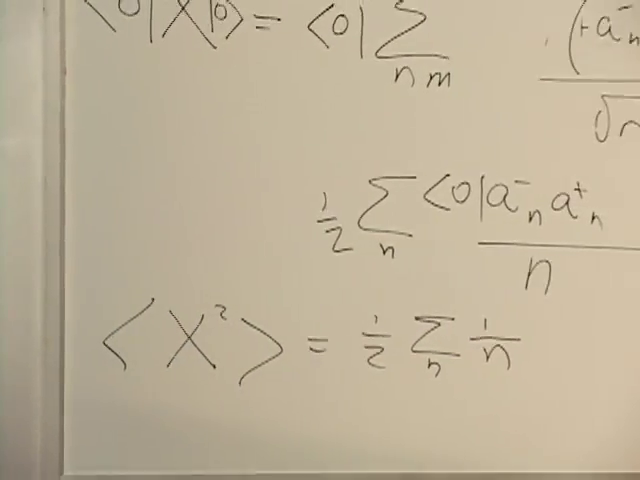
\includegraphics[width=0.72\textwidth]{lecture_09_figure_05.png}
  \caption{黑板上给出了控制基态展宽的调和求和。}
  \lectureframe{00:22:05}
  \label{fig:l09-harmonic-size}
\end{figure}

只保留比如说前二十五个模式，会得到一个有限的模糊客体，但它还不是连续弦。去掉截断会使均方展宽按对数增长。这一结论不应被误读为平直空间弦理论不自洽的证明。在平直空间中，质心运动与振子运动分离，物理振幅中精细的相消保持了预期的定域性。尺寸的增长是一个警告。曲率告诉我们这一警告是否会变成失败。

\section{当内部展宽改变几何时}

把弦放在球面的北极附近。当所有振子都被关闭时，它的行为就像刚才研究过的点粒子。随着更高模式被允许，弦变成一个在球冠上铺展开的涨落缠结。它的中心仍可绕球面运动，但进入转动能量的转动惯量所对应的客体现在是延展的。

对于穿过球心与两极的轴，
\begin{equation}
  I=\int r_\perp^2\,dm,
  \label{eq:l09-extended-inertia}
\end{equation}
其中\(r_\perp\)是弦元到该轴的垂直距离。轨道赤道处的一点具有最大的相关力臂。弦中向轴下垂的部分贡献较小。在总质量固定时，这降低了有效转动惯量：
\begin{equation}
  I_{\mathrm{eff}}<mR^2.
  \label{eq:l09-inertia-reduction}
\end{equation}
因此转动能量看起来像是一个位于更小球面上的点状客体的转动能量，
\begin{equation}
  E_{\mathrm{rot}}
  =\frac{L^2}{2I_{\mathrm{eff}}}
  \equiv \frac{L^2}{2mR_{\mathrm{eff}}^2},
  \qquad R_{\mathrm{eff}}<R.
  \label{eq:l09-effective-radius}
\end{equation}

\begin{classroomqa}
\audiencequestion{如果弦正在更大的区域上铺展开，为什么转动惯量会趋于零？\lecturetimestamp{00:33:23}}
\lecturerresponse{这一陈述是关于逐次粗粒化下的有效描述的，并不是说原始的延展分布立即具有零惯量。第一带模式把点变成一个模糊团块，其运动方式如同它生活在一个更小的球面上。下一带模式分辨出每个这样的团块内部的结构，并重复同样的重整化。迭代这一比较会把有效半径向内推。}
\end{classroomqa}

\begin{figure}[H]
  \centering
  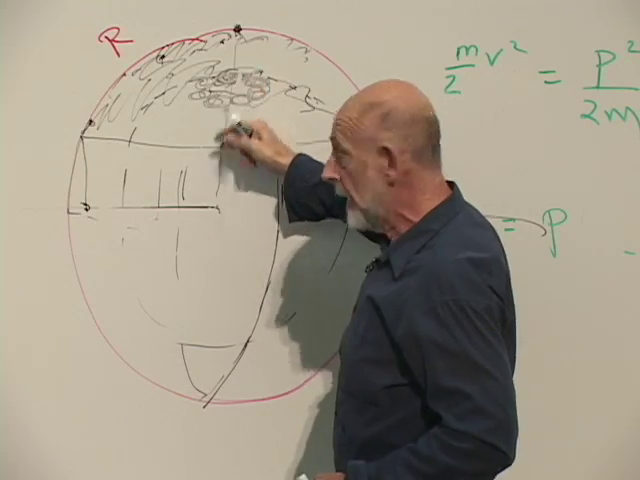
\includegraphics[width=0.72\textwidth]{lecture_09_figure_06.png}
  \medskip

  \begin{adjustbox}{max width=\linewidth}
  \begin{tikzpicture}[x=1cm,y=1cm,>=Latex]
    \draw[thick] (0,0) circle (2.15);
    \draw[dashed] (0,-2.55) -- (0,2.55);
    \draw[blue!65!black,thick]
      (-0.22,2.05)
      .. controls (-1.22,1.75) and (-1.52,1.08) .. (-1.06,0.44)
      .. controls (-0.55,-0.10) and (0.35,0.02) .. (1.10,0.68)
      .. controls (1.48,1.12) and (1.16,1.80) .. (0.20,2.05);
    \draw[red!70!black,dashed] (0,0) circle (1.25);
    \draw[->] (2.70,1.55) -- (4.05,1.55);
    \node[align=center] at (3.37,1.98) {add shorter\\modes};
    \draw[thick] (6.15,0) circle (1.25);
    \draw[dashed] (6.15,-1.65) -- (6.15,1.65);
    \draw[blue!65!black,thick]
      (6.00,1.18)
      .. controls (5.42,0.88) and (5.46,0.25) .. (6.02,-0.06)
      .. controls (6.46,-0.28) and (6.90,0.45) .. (6.28,1.18);
    \node at (0,-3.00) {sphere of radius \(R\)};
    \node at (6.15,-2.05) {effective radius \(R_{\mathrm{eff}}\)};
  \end{tikzpicture}
  \end{adjustbox}
  \caption{黑板上的北极弦以及有效半径论证的清晰重构。虚线内圆是一种有效几何，而不是球面内部的第二个物理壳层。}
  \lectureframe{00:35:15}
  \label{fig:l09-shrinking-sphere}
\end{figure}

这是一个重整化群陈述。有限截断使弦成为一个具有有限内部分辨率的团块。提高截断会改变该团块的力学。在正曲率球面上，每增加一层模式壳都会使从长距离运动推断出的背景变小。如果结果永不稳定，那么在该背景上就不存在与截断无关的弦理论。

\section{度规必须达到不动点}

现在把球面替换为一般的目标空间度规
\(g_{\mu\nu}(x)\)。在振子模式的薄对数壳层中积分会以局部对称二阶张量的形式改变该度规。这一改变必须在平直空间中消失，并且从度规的两个导数开始。在领头阶，协变性使里奇张量成为相关候选：
\begin{equation}
  \frac{\partial g_{\mu\nu}}{\partial\log\Lambda}
  =-C\,R_{\mu\nu}+\cdots ,
  \qquad C>0
  \label{eq:l09-ricci-flow}
\end{equation}
其方向对应于几何论证中所用的粗粒化方向。于是正曲率会把球面向内驱动，正如所需。
\editorialnote{归一化和符号取决于重整化参数是朝紫外还是朝红外增加。在通常的世界面记号中，领头度规贝塔函数是\(\beta^g_{\mu\nu}=\alpha'R_{\mu\nu}+\cdots\)。这里所用的不变量陈述是：截断无关性要求贝塔函数，因而在此阶要求\(R_{\mu\nu}\)，为零。}

\begin{figure}[H]
  \centering
  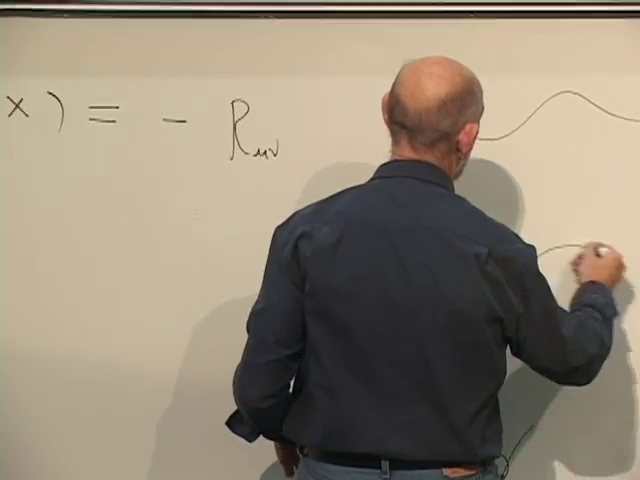
\includegraphics[width=0.76\textwidth]{lecture_09_figure_07.png}
  \caption{度规改变被示意性地写成负的里奇张量，旁边画有一条平滑曲线。}
  \lectureframe{00:43:00}
  \label{fig:l09-ricci-flow-board}
\end{figure}

\begin{classroomqa}
\audiencequestion{振子截断\(N\)在这个流方程中出现在哪里？\lecturetimestamp{00:43:38}}
\lecturerresponse{它就是标度变量。当所包含的最高模发生变化时，弦尺度求和按对数方式改变，因此自然的演化参数是\(\log N\)，或者等价地是\(\log\Lambda\)。方程\eqref{eq:l09-ricci-flow}描述了一个对数壳层模式所引起的无穷小变化。}
\end{classroomqa}

可容许的背景是这个流的不动点。在领头阶，
\begin{equation}
  \boxed{R_{\mu\nu}=0.}
  \label{eq:l09-ricci-flat}
\end{equation}
Ricci 平坦并不意味着 Riemann 张量的每一个分量都为零。例如，引力波在真空中可以具有非零曲率，同时满足\(R_{\mu\nu}=0\)。

\subsection{同一条件就是真空 Einstein 方程}

在抑制掉常规常数后，Einstein 方程为
\begin{equation}
  G_{\mu\nu}
  \equiv
  R_{\mu\nu}-\frac12 g_{\mu\nu}R
  =T_{\mu\nu}.
  \label{eq:l09-einstein}
\end{equation}

\begin{figure}[H]
  \centering
  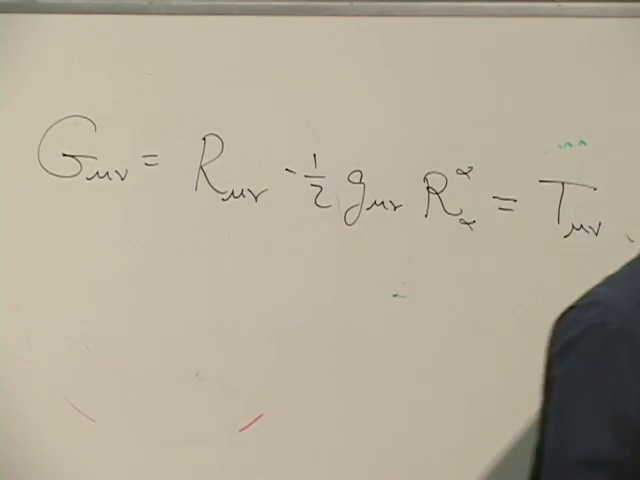
\includegraphics[width=0.78\textwidth]{lecture_09_figure_08.png}
  \caption{黑板上的 Einstein 张量与应力张量。}
  \lectureframe{00:47:15}
  \label{fig:l09-einstein-board}
\end{figure}

在真空中\(T_{\mu\nu}=0\)。在\(D\)维时空中取迹得到
\begin{equation}
  0=g^{\mu\nu}G_{\mu\nu}
   =\left(1-\frac{D}{2}\right)R.
  \label{eq:l09-einstein-trace}
\end{equation}
对于\(D\neq2\)，有\(R=0\)，再代回\eqref{eq:l09-einstein}便得到\(R_{\mu\nu}=0\)。因此，弦失去其对截断的依赖这一条件就是真空引力场方程。引力并不是被附加到理论上的；它是作为一致性的代价而出现的。

\emph{真空}一词并不意味着什么都不发生。它意味着该区域内没有应力-能量源。无源的 Maxwell 方程允许电磁波，无源的 Einstein 方程允许引力波。即使其 Ricci 张量为零，几何仍然可以是动力学的。

\begin{classroomqa}
\audiencequestion{这个条件与共形不变性有关吗？\lecturetimestamp{00:52:20}}
\lecturerresponse{是的，尽管这个问题在录音中有一部分丢失了。相关的对称性是\emph{世界面}量子理论的共形不变性。要求世界面标度反常消失，正是使度规 beta 函数为零的条件。不应把它与要求时空本身共形不变混淆起来。}
\end{classroomqa}

还有第二个一致性条件。世界面共形不变性还确定了临界时空维度：超弦为十维，玻色弦为二十六维。因此，仅 Ricci 平坦并不是全部要求，但它是最直接地显示出 Einstein 方程的那一部分。

\section{紧致维度而非缺失维度}

超弦背景有九个空间维度和一个时间维度。我们的宏观世界只显示出三个大的空间方向，因此六个空间维度必须在通常尺度下被隐藏起来，或者以其他方式变得不可及。紧致化使它们保持为真正的维度，同时赋予它们小的有限尺度。

\begin{classroomqa}
\audiencequestion{如果不同的观测者携带不同的时钟，那是否相当于拥有不止一个时间维度？\lecturetimestamp{00:56:59}}
\lecturerresponse{不。许多时钟只是许多测量一个时空中坐标的仪器；它们并不会创造出独立的类时方向。这里考虑的额外维度是空间性的。熟悉的量子构造和因果构造并不能提供一种可与之相比的、具有多个局部时间方向的一致理论，因此那种可能性不属于这个紧致化模型。}
\end{classroomqa}

想象一些生物，它们相信自己的世界是一条线。在低分辨率下，它们只能向前和向后移动。然而，在足够强大的显微镜下，这条线被揭示为一个非常细的圆柱。一个小生物除了可以沿着它的长度移动外，还可以绕着它的圆周方向移动。第二个方向一直存在；只是它的周长太小，粗糙的探测无法分辨。

\begin{figure}[H]
  \centering
  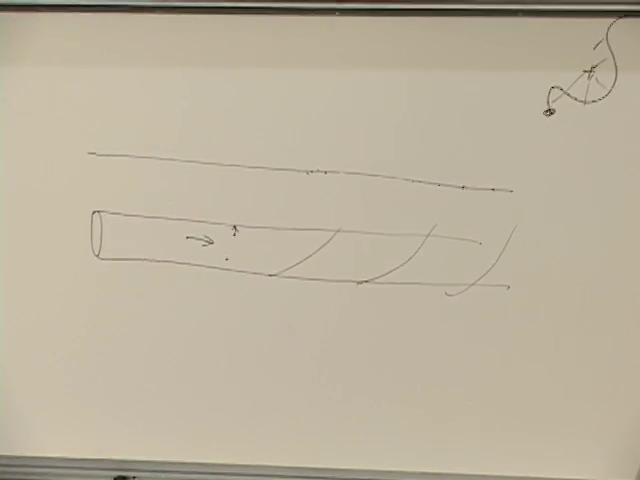
\includegraphics[width=0.78\textwidth]{lecture_09_figure_09.png}
  \caption{一个狭窄的圆柱以及绕其隐藏圆周方向缠绕的轨迹。}
  \lectureframe{01:01:00}
  \label{fig:l09-hidden-cylinder}
\end{figure}

圆柱可以表示为一个带，其上边缘和下边缘被等同起来。穿过上边缘会从下边缘的同一纵向位置返回。两个边缘处都没有物理边界。同样的操作可以用两个方向来进行：把一个矩形的左边缘和右边缘等同起来，同时也把它的上边缘和下边缘等同起来。结果就是一个二维环面。

\begin{figure}[H]
  \centering
  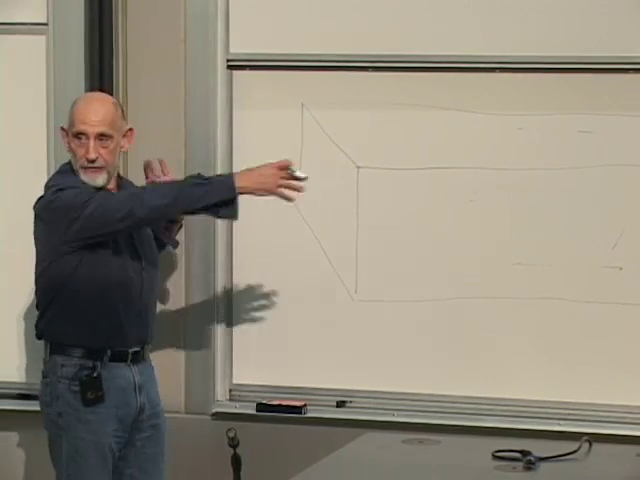
\includegraphics[width=0.76\textwidth]{lecture_09_figure_10.png}
  \medskip

  \begin{tikzpicture}[x=0.82cm,y=0.82cm,>=Latex]
    \draw[thick] (0,0) rectangle (4,2.15);
    \draw[blue!65!black,->] (0,2.48) -- (4,2.48);
    \draw[blue!65!black,->] (4,-0.34) -- (0,-0.34);
    \node at (2,-0.82) {one periodic direction};
    \draw[thick] (6.1,0) rectangle (10.1,2.15);
    \draw[blue!65!black,->] (6.1,2.48) -- (10.1,2.48);
    \draw[blue!65!black,->] (10.1,-0.34) -- (6.1,-0.34);
    \draw[red!70!black,->] (5.76,0) -- (5.76,2.15);
    \draw[red!70!black,->] (10.44,2.15) -- (10.44,0);
    \node at (8.1,-0.82) {two periodic directions};
  \end{tikzpicture}
  \caption{黑板上的板条以及一个干净的基本区域描述。等同一对边缘得到圆柱；等同两对边缘得到环面。}
  \lectureframe{01:04:40}
  \label{fig:l09-periodic-identification}
\end{figure}

环面首先是一种拓扑，其次才是三维空间中形如面包圈的曲面。把环面剪一刀，它就变成一个圆柱面；再剪一刀，它就变成一个矩形，前提是记住边的粘合方式。可以在这个矩形上放置一个平坦度规，因此所得的平坦环面局部具有零黎曼曲率，当然也是里奇平坦的。

矩形上的一条直线轨迹穿过一条被粘合的边后仍保持直线。如果它的斜率是两个周期的有理比，轨迹最终会闭合。如果这个比是无理数，它就永不闭合，并会在环面上变得稠密。

\begin{figure}[H]
  \centering
  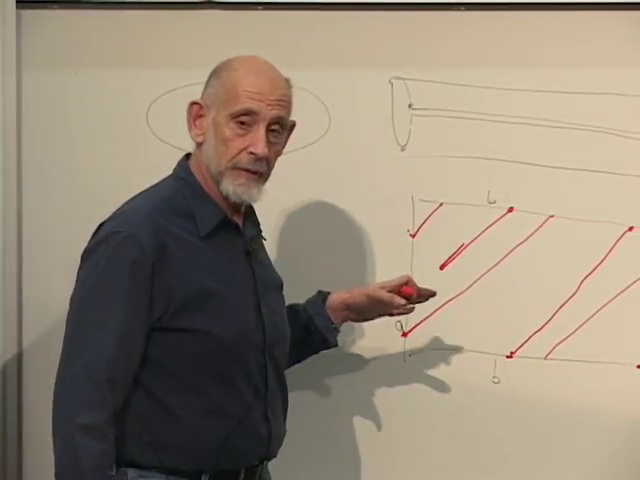
\includegraphics[width=0.76\textwidth]{lecture_09_figure_11.png}
  \caption{基本域中反复出现的直线段代表环面上的一条不间断轨迹。}
  \lectureframe{01:11:00}
  \label{fig:l09-torus-trajectory}
\end{figure}

高维环面以同样的方式构成。把立方体的每一对相对面粘合起来就得到一个三环面，而六个紧致方向可以用一个六环面来建模。不应试图把所有这些对象都嵌入普通的三维空间；面粘合的描述是内蕴的，也是完备的。

\begin{classroomqa}
\audiencequestion{额外维度是否必然要卷回到自身？
\lecturetimestamp{01:15:03}}
\lecturerresponse{并非作为一条定理。它也可以是非紧致的，但那样它通常会作为观测到的长距离世界中的另一个大方向而出现。紧致性是使额外维度与其表面上的缺失相协调的最简单方式。自然界为何选择某种特定的紧致化，则是一个独立的动力学问题。}
\end{classroomqa}

\begin{classroomqa}
\audiencequestion{为什么要假设那些看不见的维度是以这种方式卷曲起来的普通空间方向，而不是某种完全不同的东西？\lecturetimestamp{01:15:51}}
\lecturerresponse{因为这是一个确定的、可求解的假设，而不是因为它已被证明是对自然界的唯一描述。紧致空间流形使我们能够构造自洽的例子并计算其谱。更奇异的可能性必须通过做到同样的事情来赢得自己的位置。}
\end{classroomqa}

\begin{classroomqa}
\audiencequestion{熟悉的面包圈形环面上的距离看起来并不像矩形中的距离。这里指的是哪一种几何？
\lecturetimestamp{01:18:11}}
\lecturerresponse{\emph{环面}一词固定的是粘合方式，而不是某一个唯一的度规。嵌入的面包圈从三维空间继承了一个弯曲度规。周期粘合的矩形则带有一个平坦度规。它们具有相同的拓扑和不同的几何；对于这里所说的简单紧致化，我们指的是平坦的那一个。}
\end{classroomqa}

\section{平坦环面的形状参数}

即便是一个平坦的二环面也不是唯一的。它的基本平行四边形有一个总面积、一个长宽比和一个剪切。改变这些参数会改变距离，从而改变谱，但不改变拓扑。

\begin{figure}[H]
  \centering
  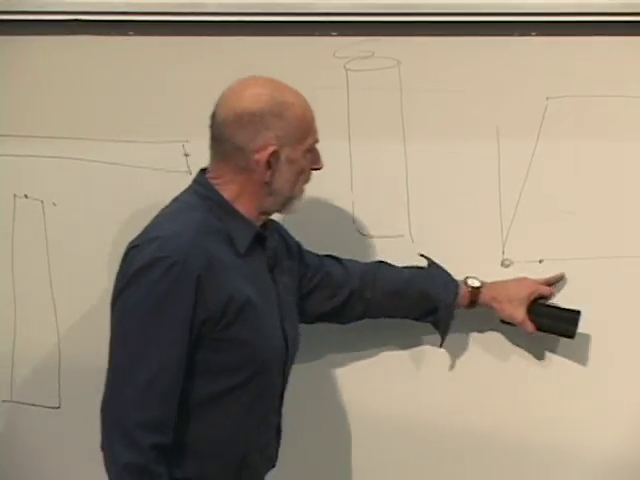
\includegraphics[width=0.74\textwidth]{lecture_09_figure_12.png}
  \medskip

  \begin{tikzpicture}[x=0.9cm,y=0.9cm,>=Latex]
    \draw[thick] (0,0) rectangle (3.4,2.1);
    \draw[<->] (0,-0.35) -- node[below] {\(L_1\)} (3.4,-0.35);
    \draw[<->] (-0.35,0) -- node[left] {\(L_2\)} (-0.35,2.1);
    \draw[thick] (5.4,0) -- (8.8,0) -- (9.7,2.1) -- (6.3,2.1) -- cycle;
    \draw[dashed] (5.4,0) -- (6.3,2.1);
    \draw[->] (5.75,2.48) -- node[above] {shear} (6.45,2.48);
    \node at (1.7,-1.00) {area and aspect ratio};
    \node at (7.55,-1.00) {complex structure};
  \end{tikzpicture}
  \caption{用于讨论环面模数的矩形基本域和剪切基本域。}
  \lectureframe{01:23:00}
  \label{fig:l09-torus-moduli}
\end{figure}

对于二环面，把形状打包成一个复数\(\tau=\tau_1+i\tau_2\)是有用的：实部记录剪切，虚部在分离出整体标度后记录长宽比。交换两个基本循环或改变它们的整数基，可以使表面上不同的平行四边形描述同一个环面。

\begin{classroomqa}
\audiencequestion{如果在粘合之前把一条边翻转，会发生什么？\lecturetimestamp{01:24:20}}
\lecturerresponse{那会产生一种不同的拓扑。用反射来粘合会得到一个不可定向曲面，即克莱因瓶，而不是普通的环面。}
\end{classroomqa}

\begin{classroomqa}
\audiencequestion{如果扭转沿边不是均匀的呢？
\lecturetimestamp{01:25:01}}
\lecturerresponse{一个光滑的非均匀形变可以被转移到基本域上的度规中。拓扑粘合与几何数据必须保持区分：改变粘合方式可能改变拓扑，而光滑地改变距离则改变度规。}
\end{classroomqa}

\editorialnote{对于平坦二环面，面积是最简单的凯勒模数，而\(\tau\)是复结构模数。连续的剪切是\(\tau\)的一部分。德恩扭转则是一种离散的映射类操作，由\(\tau\mapsto\tau+1\)表示；它本身并不是那个连续模数。这澄清了黑板讨论中所使用的有意非正式的术语。}

平坦环面之所以有用，是因为它们立即满足自洽性条件，但它们的对称性对于粒子物理的现实模型来说过于宽裕。更精细的里奇平坦空间，尤其是卡拉比--丘流形，提供了更丰富的紧致化。它们的详细构造超出了本讨论的范围；原理仍然相同。

\section{从谱中读出紧致圆}

休息之后，把紧致空间约化为一个周长为
\(2\pi R\)的圆。波函数绕行一周后必须单值：
\begin{equation}
  e^{ip_c(x+2\pi R)/\hbar}=e^{ip_cx/\hbar}.
\end{equation}
因此
\begin{equation}
  p_cR=n\hbar,
  \qquad
  p_c=\frac{n\hbar}{R},
  \qquad n\in\mathbb Z.
  \label{eq:l09-kk-momentum}
\end{equation}

\begin{figure}[H]
  \centering
  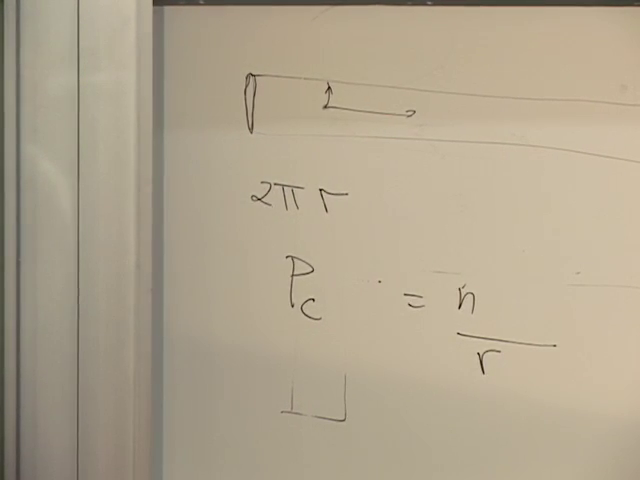
\includegraphics[width=0.74\textwidth]{lecture_09_figure_13.png}
  \caption{紧致周长\(2\pi R\)与量子化动量
  \(p_c=n\hbar/R\)。}
  \lectureframe{01:32:15}
  \label{fig:l09-kk-board}
\end{figure}

对于全时空中的无质量粒子，
\begin{equation}
  E=c|\mathbf P|.
  \label{eq:l09-massless-dispersion}
\end{equation}

\begin{figure}[H]
  \centering
  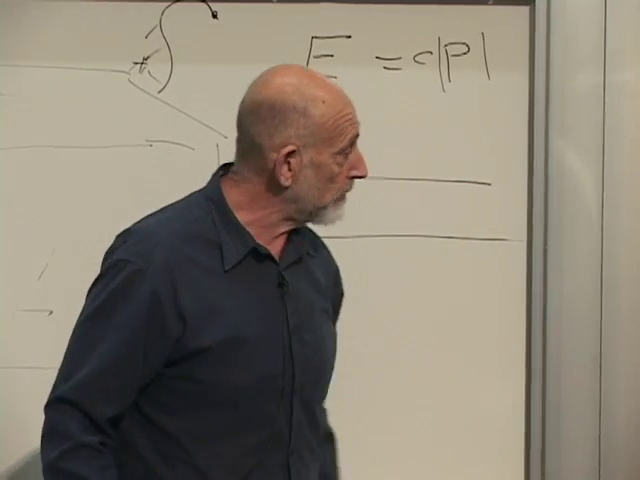
\includegraphics[width=0.70\textwidth]{lecture_09_figure_14.png}
  \caption{用于把紧致动量重新解释为低维质量的无质量色散关系。}
  \lectureframe{01:33:45}
  \label{fig:l09-massless-board}
\end{figure}

把动量分成非紧致部分与紧致部分，并令
\(c=\hbar=1\)：
\begin{equation}
  E^2=\mathbf p_{\mathrm{large}}^2+\frac{n^2}{R^2}.
  \label{eq:l09-kk-dispersion}
\end{equation}
无法分辨紧致方向的观测者将它与
\(E^2=\mathbf p_{\mathrm{large}}^2+m^2\)相比较，推断出一系列质量
\begin{equation}
  m_n=\frac{|n|}{R}.
  \label{eq:l09-kk-masses}
\end{equation}
\(n\)的两个符号描述的是具有相同正能量的相反紧致动量，而不是正质量和负质量。因此，间距\(1/R\)通过光谱揭示了半径。这就是
Kaluza--Klein机制：隐藏方向上的动量在可见维度中表现为质量。

\section{缠绕态补全谱}

闭弦具有一种点粒子不具备的可能性：它可以缠绕在圆上。若缠绕数为\(w\)，则弦只有在绕紧致方向\(w\)圈后才闭合。其长度为
\(2\pi |w|R\)，因此张力提供能量
\begin{equation}
  m_w
  =2\pi T\,|w|R
  =\frac{|w|R}{\alpha'}.
  \label{eq:l09-winding-mass}
\end{equation}
本讲选取\(\alpha'=1\)的单位，将其约化为
\begin{equation}
  m_w=|w|R.
  \label{eq:l09-winding-lecture-units}
\end{equation}
正的和负的\(w\)是绕圆的相反取向。

\begin{figure}[H]
  \centering
  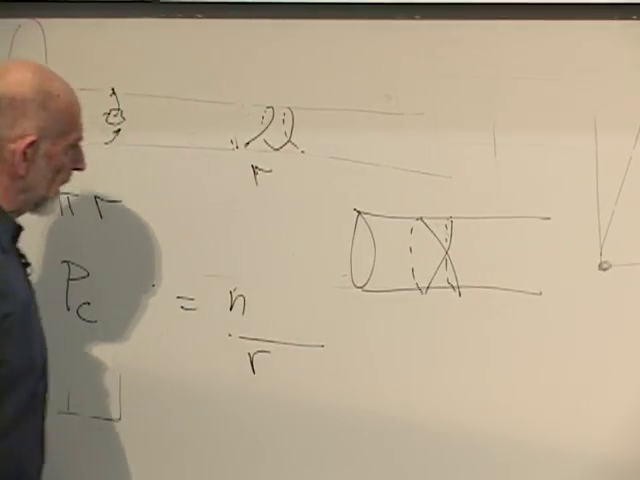
\includegraphics[width=0.76\textwidth]{lecture_09_figure_15.png}
  \caption{缠绕在紧致圆柱上的闭弦，黑板上标出了紧致半径。}
  \lectureframe{01:39:45}
  \label{fig:l09-winding-board}
\end{figure}

因此，紧致圆产生两个互补的阶梯：
\begin{equation}
  m_n=\frac{|n|}{R},
  \qquad
  m_w=\frac{|w|R}{\alpha'}.
  \label{eq:l09-two-towers}
\end{equation}
当\(R\)大时，动量能级间距小，而缠绕态很重。当\(R\)小时，动量能级间距大，而缠绕态很轻。

\begin{figure}[H]
  \centering
  \begin{tikzpicture}[x=1cm,y=0.9cm,>=Latex]
    \draw[->] (0,0) -- (0,4.7) node[above] {\(m\)};
    \foreach \y/\lab in {0/0,1.1/{1/R},2.2/{2/R},3.3/{3/R},4.4/{4/R}} {
      \draw (-0.16,\y) -- (0.16,\y);
      \node[left] at (-0.22,\y) {\(\lab\)};
    }
    \node at (0,-0.62) {momentum};
    \draw[<->,very thick,blue!65!black] (2.05,2.15) -- (4.05,2.15)
      node[midway,above] {\(R\leftrightarrow\alpha'/R\)};
    \draw[->] (6.1,0) -- (6.1,4.7) node[above] {\(m\)};
    \foreach \y/\lab in {0/0,1.1/{R/\alpha'},2.2/{2R/\alpha'},3.3/{3R/\alpha'},4.4/{4R/\alpha'}} {
      \draw (5.94,\y) -- (6.26,\y);
      \node[right] at (6.32,\y) {\(\lab\)};
    }
    \node at (6.1,-0.62) {winding};
  \end{tikzpicture}
  \caption{当半径以弦单位取倒数时，动量阶梯与缠绕阶梯互换。}
  \label{fig:l09-dual-mass-towers}
\end{figure}

\section{T对偶：小圆与大圆是相同的物理}

两个阶梯通过
\begin{equation}
  R\longleftrightarrow\frac{\alpha'}{R},
  \qquad
  n\longleftrightarrow w.
  \label{eq:l09-t-duality}
\end{equation}互换。
在黑板上所用的单位中，\(\alpha'=1\)，因此这简单地就是
\(R\leftrightarrow1/R\)。在自对偶半径
\(R=\sqrt{\alpha'}\)处，动量标度与缠绕标度重合。

\begin{figure}[H]
  \centering
  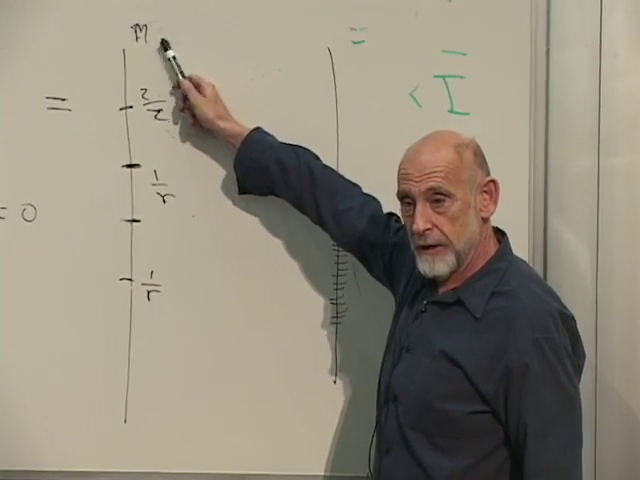
\includegraphics[width=0.74\textwidth]{lecture_09_figure_16.png}
  \caption{黑板上比较了半径越过自对偶标度时稀疏与稠密的质量阶梯。}
  \lectureframe{01:43:00}
  \label{fig:l09-duality-board}
\end{figure}

基本质量公式的互换只是这一结果可见的边缘。闭弦振子态与散射振幅也被一致地映射。比弦标度更小的圆并不是一种新的、越来越小的几何；它有一个作为更大对偶圆的等价描述。点粒子无法作出这种等同，因为它们拥有动量模但没有缠绕模。

\begin{classroomqa}
\audiencequestion{这难道仅仅等同于交换一个竖直方向和一个水平方向吗？\lecturetimestamp{01:44:38}}
\lecturerresponse{不。它交换的是两个不同的量子数：绕圆的动量与闭弦缠绕圆的次数。半径必须同时取倒数。}
\end{classroomqa}

\begin{classroomqa}
\audiencequestion{在\(R<\sqrt{\alpha'}\)和
\(R>\sqrt{\alpha'}\)处的描述只涉及玻色子，还是也涉及费米子？
\lecturetimestamp{01:46:30}}
\lecturerresponse{这种对偶性是整个紧致化弦理论的对称性，而不只是用来揭示它的简单玻色子质量阶梯的对称性。各扇区的详细映射取决于理论，但小--大的等价性并不限于一种粒子。}
\end{classroomqa}

\begin{classroomqa}
\audiencequestion{所比较的两个态是开弦还是闭弦？\lecturetimestamp{01:47:32}}
\lecturerresponse{它们是闭弦态。自由传播的闭弦可以缠绕紧致圆。端点自由的普通开弦不携带同样的守恒缠绕数。}
\end{classroomqa}
\editorialnote{在更完整的开弦论述中，T对偶交换Neumann边界条件与Dirichlet边界条件，并引入D膜。这就是为什么开弦的T对偶比简单照搬闭弦缠绕公式更为丰富。}

\begin{classroomqa}
\audiencequestion{这种互换是否类似于黑洞视界附近空间与时间的交换？\lecturetimestamp{01:48:00}}
\lecturerresponse{不是。视界坐标与因果性质是另一个不同的问题。这里两种描述涉及的是同一个紧致空间圆以及其动量扇区与缠绕扇区的交换。}
\end{classroomqa}

\begin{classroomqa}
\audiencequestion{这是否通过给出一个最小长度而解决了短距离自能问题？\lecturetimestamp{01:48:35}}
\lecturerresponse{它表明，小于弦尺度的半径并不定义新的不等价的圆背景：将\(R\)减小到自对偶点以下会增大对偶半径。这是对探测任意小圆几何的一种精确的弦论障碍，尽管不应把它变成这样一种主张：每一个可以想象的距离概念都有一个普适的硬性下界。}
\end{classroomqa}

\section{为什么缠绕扇区不能被省略}

\begin{classroomqa}
\audiencequestion{我们能否只用未缠绕的弦来定义理论，而把缠绕态排除在外？\lecturetimestamp{01:48:56}}
\lecturerresponse{不能。闭弦相互作用会产生它们。把一个未缠绕的圈沿紧致方向拉伸，使得一段沿一个方向绕圆，另一段沿相反方向绕圆。净缠绕仍然为零。随后一次重联可以把该圈分裂成两个闭弦，其缠绕数分别为\(+1\)和\(-1\)。这一对可以分开，因此即使初始态没有缠绕态，缠绕态也必须属于谱。}
\end{classroomqa}

\begin{figure}[H]
  \centering
  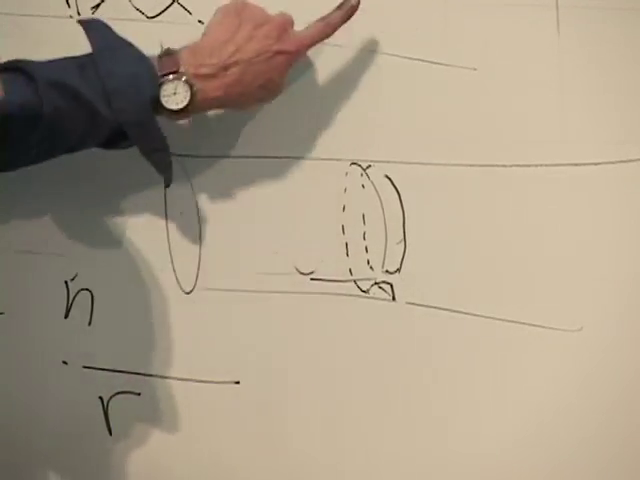
\includegraphics[width=0.74\textwidth]{lecture_09_figure_17.png}
  \caption{重联前围绕紧致方向排列的拉伸的零缠绕圈。}
  \lectureframe{01:50:30}
  \label{fig:l09-winding-pair-before}
\end{figure}

\begin{figure}[H]
  \centering
  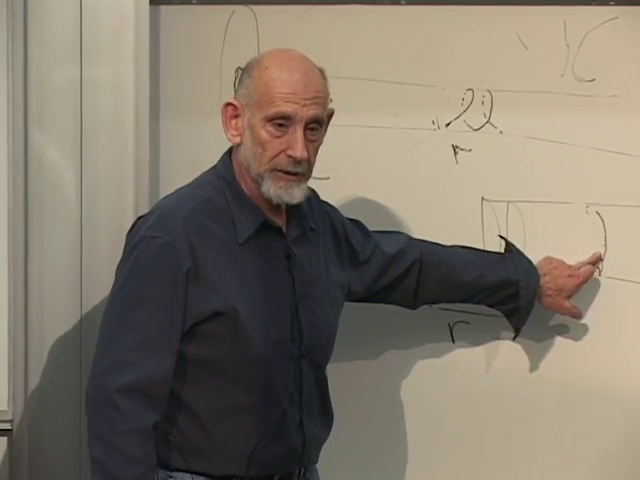
\includegraphics[width=0.72\textwidth]{lecture_09_figure_18.png}
  \medskip

  \begin{tikzpicture}[x=0.9cm,y=0.9cm,>=Latex]
    \draw[thick] (0,0) ellipse (1.0 and 1.55);
    \draw[blue!65!black,thick]
      (0.08,1.35) .. controls (2.0,1.15) and (2.0,-1.15) .. (0.08,-1.35);
    \draw[red!70!black,thick]
      (-0.08,-1.35) .. controls (-2.0,-1.15) and (-2.0,1.15) .. (-0.08,1.35);
    \node at (0,-2.15) {net \(w=0\)};
    \draw[->,thick] (2.45,0) -- (3.75,0) node[midway,above] {split};
    \draw[thick] (5.05,0.62) ellipse (0.68 and 1.02);
    \draw[blue!65!black,very thick,->]
      (5.05,1.64) arc[start angle=90,end angle=-250,x radius=0.68,y radius=1.02];
    \node at (5.05,-0.82) {\(w=+1\)};
    \draw[thick] (7.45,0.62) ellipse (0.68 and 1.02);
    \draw[red!70!black,very thick,<-]
      (7.45,1.64) arc[start angle=90,end angle=-250,x radius=0.68,y radius=1.02];
    \node at (7.45,-0.82) {\(w=-1\)};
  \end{tikzpicture}
  \caption{黑板上分开的缠绕圈以及缠绕--反缠绕对产生的清晰重构。总缠绕保持为零。}
  \lectureframe{01:51:30}
  \label{fig:l09-winding-pair-after}
\end{figure}

\begin{classroomqa}
\audiencequestion{产生缠绕对是否需要额外能量？\lecturetimestamp{01:52:11}}
\lecturerresponse{需要。拉伸一根弦要付出张力能量，而最终缠绕的弦具有\eqref{eq:l09-winding-mass}中的质量。一次能量足够高的碰撞可以产生这一对，正如一次碰撞可以产生一个粒子及其反粒子，同时保持相关的守恒荷。}
\end{classroomqa}

\section{人能听出弦背景的形状吗？}

对于普通的紧致化粒子理论，Kaluza--Klein谱的间距让我们推断半径：人们试图从其简正模听出紧致空间的形状。弦理论使这个逆问题变得更加微妙。动量模听到\(1/R\)，缠绕模听到\(R/\alpha'\)，而当两者互换时，完整谱保持不变。点粒子几何视为不同的两个半径，其实是用对偶变量描述的同一个弦背景。

因此，本讲通过一条途径得出了它所承诺的两个结论。紫外一致性迫使靶空间度规满足真空爱因斯坦方程，所以引力不可避免。紧致化随后把隐藏的几何变成粒子谱，但缠绕态阻止该谱在弦尺度以下指定一个唯一的经典半径。一致性不仅仅选择哪些几何是允许的；通过T对偶，它改变了什么才算作不同的几何。
